\section{Data Description} \label{section:datadesc}
The data we will be working with in this project will come directly from \siemens. Although this data is not public, we have been allowed to use it in this project, and additionally put the full spreadsheet in appendix \ref{appendix:local-agreements}.

What we have received is a spreadsheet from the Human Resources (HR) department on the local \siemens facility in Aalborg. This department produces a schedule that needs to be looked over by a worker, to ensure that the schedule follows all union agreements. The spreadsheet from HR comes noted with what holidays and SH-days there are, but shifts are not accommodated in this spreadsheet. It is therefore the responsibility of the worker fixing the schedule to:

\begin{itemize}
    \item Accommodate holidays
    \item Accommodate SH-days
    \item Plan 3 weeks vacation in the summertime
    \item Plan 1 week vacation around Christmas
    \item Finally, make sure that all teams have their planned hours according to the union agreement
\end{itemize}

\begin{figure}[ht!]
    \centering
    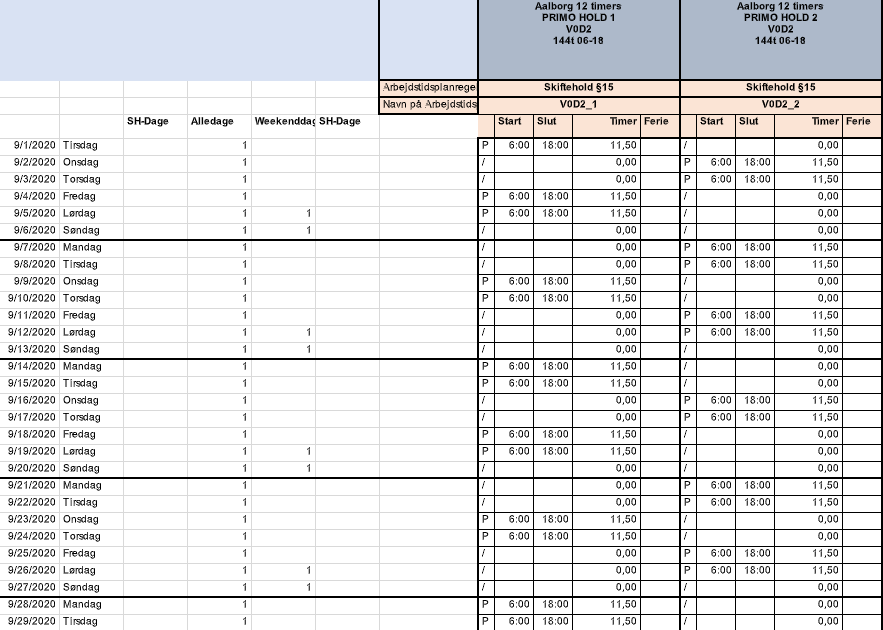
\includegraphics[width=\textwidth]{media/Schedule WO fix.png}
    \caption{Schedule that the planner receives, and then has to turn into a real schedule.}
    %first draft of the schedule proposed by Human Resources
    \label{fig:Schedule no fix}
\end{figure}

The schedule that comes in has the same structure as the example given in table \ref{tab:exampleSchedule} which can be found on page \pageref{tab:exampleSchedule}. The schedule has four teams, two day shift, and two night shift teams. We will primarily be focusing on the day shift teams, but if there is enough time we will try to make the program able to also fix the scheduling for the night shift teams. The day shift team will from here on out be called \primo team 1 and 2.


\primo team 1, as an example, works two days 6am-6pm, and then they have two days off. In those two days off, \primo team 2 works instead, which allows for production everyday, with time off. This however does not work out with a seven day work week, which is why these teams work six day work weeks. This explains why the schedule is called a 144h as well.


In figure \ref{fig:Schedule no fix} you can see the schedule given to the worker fixing it. This spreadsheet goes down 365 cells, for all the days until the next schedule needs to be. In figure \ref{fig:Schedule formated} you can see the fully formatted schedule, which is how we want the schedule to end up. This is because this is how the workers have come to expect their schedule.

\begin{figure}[ht!]
    \centering
    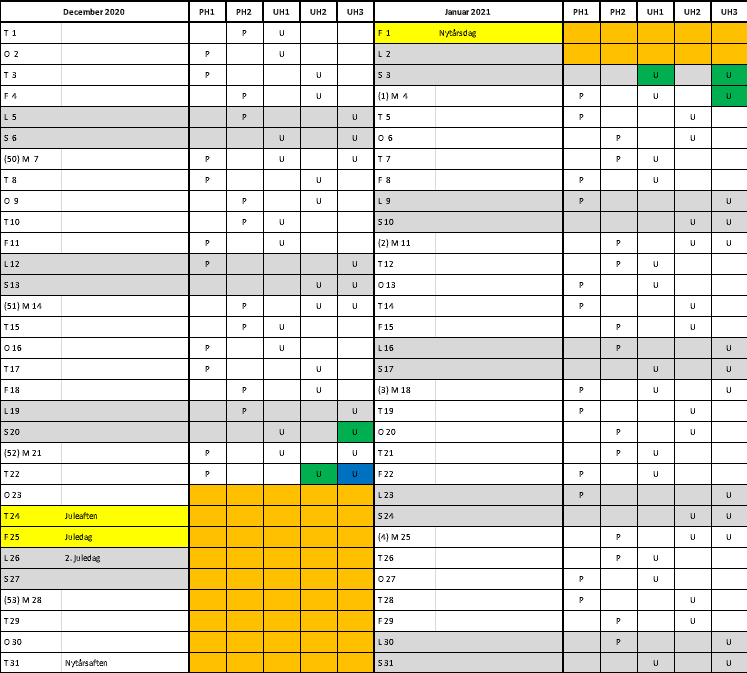
\includegraphics[width=\textwidth]{media/Schedule formated.png}
    \caption{Schedule after the planner has formatted it.}
    %Template for the final version of the schedule
    \label{fig:Schedule formated}
\end{figure}



\iffalse

The data is a spreadsheet that comes in directly from the Human Resources department. The spreadsheet has the same layout as seen in table \ref{tab:exampleSchedule} which can be found on page \pageref{tab:exampleSchedule}. Additionally the spreadsheet comes with small inputs directly from the local agreement, which helps the worker fixing the schedule, so they easily can reference different numbers like maximum hours per week.

At the end of the project, we want to create a C program that accepts the spreadsheet as a 'Semicolon-separated values'-file (\verb|.csv|), and output one as well. The program would analyse the data, see what worker shifts it should add or remove, and finally it should print it out as a schedule that is easy for the workers working the shifts to understand.

\fi
